\documentclass[12pt,twoside]{report}
\usepackage{tikz}
\usetikzlibrary{positioning, fit, arrows.meta}
\usepackage{amsmath,amssymb}

 
\usepackage{listings}
\usepackage{color}
 
\definecolor{codegreen}{rgb}{0,0.6,0}
\definecolor{codegray}{rgb}{0.5,0.5,0.5}
\definecolor{codepurple}{rgb}{0.58,0,0.82}
\definecolor{backcolour}{rgb}{0.95,0.95,0.92}
 
\lstdefinestyle{mystyle}{
    backgroundcolor=\color{backcolour},   
    commentstyle=\color{codegreen},
    keywordstyle=\color{magenta},
    numberstyle=\tiny\color{codegray},
    stringstyle=\color{codepurple},
    basicstyle=\ttfamily\footnotesize,
    breakatwhitespace=true,         
    breaklines=true,                 
    captionpos=b,                    
    keepspaces=true,                 
    numbers=left,                    
    numbersep=5pt,                  
    showspaces=false,                
    showstringspaces=false,
    showtabs=false,                  
    tabsize=2
}
 
\lstset{style=mystyle}

%%%%%%%%%%%%%%%%%%%%%%%%%%%%%%%%%%%%%%%%%%%%%%%%%%%%%%%%%%%%%%%%%%%%%%%%%%%%%

% Definitions for the title page
% Edit these to provide the correct information
% e.g. \newcommand{\reportauthor}{Timothy Kimber}

\newcommand{\reporttitle}{Chameleon Text: Exploring ways to increase variety in artificial data}
\newcommand{\reportauthor}{Thien P. Nguyen}
\newcommand{\supervisor}{Julia Ive}
\newcommand{\degreetype}{Computing (Machine Learning)}

%%%%%%%%%%%%%%%%%%%%%%%%%%%%%%%%%%%%%%%%%%%%%%%%%%%%%%%%%%%%%%%%%%%%%%%%%%%%%

% load some definitions and default packages
%%%%%%%%%%%%%%%%%%%%%%%%%%%%%%%%%%%%%%%%%
% University Assignment Title Page 
% LaTeX Template
% Version 1.0 (27/12/12)
%
% This template has been downloaded from:
% http://www.LaTeXTemplates.com
%
% Original author:
% WikiBooks (http://en.wikibooks.org/wiki/LaTeX/Title_Creation)
%
% License:
% CC BY-NC-SA 3.0 (http://creativecommons.org/licenses/by-nc-sa/3.0/)
% 
%
%%%%%%%%%%%%%%%%%%%%%%%%%%%%%%%%%%%%%%%%%
%----------------------------------------------------------------------------------------
%	PACKAGES AND OTHER DOCUMENT CONFIGURATIONS
%----------------------------------------------------------------------------------------
\usepackage[a4paper,hmargin=2.3cm,vmargin=2.0cm,includeheadfoot]{geometry}
\usepackage{textpos}
\usepackage{natbib} % for bibliography
\usepackage{tabularx,longtable,multirow,subfigure,caption}%hangcaption
\usepackage{fncylab} %formatting of labels
\usepackage{fancyhdr} % page layout
\usepackage{url} % URLs
\usepackage[english]{babel}
\usepackage{amsmath}
\usepackage{graphicx}
\usepackage{dsfont}
\usepackage{epstopdf} % automatically replace .eps with .pdf in graphics
\usepackage{backref} % needed for citations
\usepackage{array}
\usepackage{latexsym}
\usepackage[pdftex,pagebackref,hypertexnames=false,colorlinks]{hyperref} % provide links in pdf

\hypersetup{pdftitle={},
  pdfsubject={}, 
  pdfauthor={},
  pdfkeywords={}, 
  pdfstartview=FitH,
  pdfpagemode={UseOutlines},% None, FullScreen, UseOutlines
  bookmarksnumbered=true, bookmarksopen=true, colorlinks,
    citecolor=black,%
    filecolor=black,%
    linkcolor=black,%
    urlcolor=black}

\usepackage[all]{hypcap}


%\usepackage{color}
%\usepackage[tight,ugly]{units}
%\usepackage{float}
%\usepackage{tcolorbox}
%\usepackage[colorinlistoftodos]{todonotes}
% \usepackage{ntheorem}
% \theoremstyle{break}
% \newtheorem{lemma}{Lemma}
% \newtheorem{theorem}{Theorem}
% \newtheorem{remark}{Remark}
% \newtheorem{definition}{Definition}
% \newtheorem{proof}{Proof}


%%% Default fonts
\renewcommand*{\rmdefault}{bch}
\renewcommand*{\ttdefault}{cmtt}



%%% Default settings (page layout)
\setlength{\parindent}{0em}  % indentation of paragraph

\setlength{\headheight}{14.5pt}
\pagestyle{fancy}
\renewcommand{\chaptermark}[1]{\markboth{\chaptername\ \thechapter.\ #1}{}} 

\fancyfoot[ER,OL]{\sffamily\textbf{\thepage}}%Page no. in the left on odd pages and on right on even pages
\fancyfoot[OC,EC]{\sffamily }
\renewcommand{\headrulewidth}{0.1pt}
\renewcommand{\footrulewidth}{0.1pt}
\captionsetup{margin=10pt,font=small,labelfont=bf}


%--- chapter heading

\def\@makechapterhead#1{%
  \vspace*{10\p@}%
  {\parindent \z@ \raggedright \sffamily
    \interlinepenalty\@M
    \Huge\bfseries \thechapter \space\space #1\par\nobreak
    \vskip 30\p@
  }}

%---chapter heading for \chapter*  
\def\@makeschapterhead#1{%
  \vspace*{10\p@}%
  {\parindent \z@ \raggedright
    \sffamily
    \interlinepenalty\@M
    \Huge \bfseries  #1\par\nobreak
    \vskip 30\p@
  }}

\allowdisplaybreaks

% load some macros
% Here, you can define your own macros. Some examples are given below.

\newcommand{\R}[0]{\mathds{R}} % real numbers
\newcommand{\Z}[0]{\mathds{Z}} % integers
\newcommand{\N}[0]{\mathds{N}} % natural numbers
\newcommand{\C}[0]{\mathds{C}} % complex numbers
\renewcommand{\vec}[1]{{\boldsymbol{{#1}}}} % vector
\newcommand{\mat}[1]{{\boldsymbol{{#1}}}} % matrix


\date{May 2019}

\begin{document}

% load title page
% Last modification: 2015-08-17 (Marc Deisenroth)
\begin{titlepage}

\newcommand{\HRule}{\rule{\linewidth}{0.5mm}} % Defines a new command for the horizontal lines, change thickness here


%----------------------------------------------------------------------------------------
%	LOGO SECTION
%----------------------------------------------------------------------------------------


\includegraphics[width = 4cm]{./figures/imperial}\\[0.5cm] 

\center % Center remainder of the page

%----------------------------------------------------------------------------------------
%	HEADING SECTIONS
%----------------------------------------------------------------------------------------

\textsc{\Large Imperial College London}\\[0.5cm] 
\textsc{\large Department of Computing}\\[0.5cm] 

%----------------------------------------------------------------------------------------
%	TITLE SECTION
%----------------------------------------------------------------------------------------

\HRule \\[0.4cm]
{ \huge \bfseries \reporttitle}\\ % Title of your document
\HRule \\[1.5cm]
 
%----------------------------------------------------------------------------------------
%	AUTHOR SECTION
%----------------------------------------------------------------------------------------

\begin{minipage}{0.4\textwidth}
\begin{flushleft} \large
\emph{Author:}\\
\reportauthor % Your name
\end{flushleft}
\end{minipage}
~
\begin{minipage}{0.4\textwidth}
\begin{flushright} \large
\emph{Supervisor:} \\
\supervisor % Supervisor's Name
\end{flushright}
\end{minipage}\\[4cm]


%----------------------------------------------------------------------------------------
%	FOOTER & DATE SECTION
%----------------------------------------------------------------------------------------
\vfill % Fill the rest of the page with whitespace
Submitted in partial fulfillment of the requirements for the MSc degree in
\degreetype~of Imperial College London\\[0.5cm]

\makeatletter
\@date 
\makeatother


\end{titlepage}



% page numbering etc.
\pagenumbering{roman}
\clearpage{\pagestyle{empty}\cleardoublepage}
\setcounter{page}{1}
\pagestyle{fancy}

%%%%%%%%%%%%%%%%%%%%%%%%%%%%%%%%%%%%
\begin{abstract}


% While recent neural encoder-decoder models have shown great promise in mod- eling open-domain conversations, they often generate dull and generic responses. Unlike past work that has focused on diversifying the output of the decoder at word-level to alleviate this problem, we present a novel framework based on conditional variational autoencoders that captures the discourse-level diversity in the encoder. Our model uses latent vari- ables to learn a distribution over potential conversational intents and generates diverse responses using only greedy de- coders. We have further developed a novel variant that is integrated with linguistic prior knowledge for better performance. Finally, the training procedure is improved by introducing a bag-of-word loss. Our proposed models have been validated to generate significantly more diverse responses than baseline approaches and exhibit competence in discourse-level decision-making.

% Combining the virtues of probability graphic models and neural networks, Conditional Variational Auto-encoder (CVAE) has shown promising performance in many applications such as response generation. However, ex- isting CVAE-based models often generate re- sponses from a single latent variable which may not be sufficient to model high variabil- ity in responses. To solve this problem, we propose a novel model that sequentially in- troduces a series of latent variables to con- dition the generation of each word in the re- sponse sequence. In addition, the approxi- mate posteriors of these latent variables are augmented with a backward Recurrent Neural Network (RNN), which allows the latent vari- ables to capture long-term dependencies of fu- ture tokens in generation. To facilitate train- ing, we supplement our model with an auxil- iary objective that predicts the subsequent bag of words. Empirical experiments conducted on the OpenSubtitle and Reddit datasets show that the proposed model leads to significant improvements on both relevance and diversity over state-of-the-art baselines.

Variational autoencoders (VAEs) have shown a lot of promise in other machine learning fields but are relatively unexplored in comparison to their potential applications as a language model. We explore the potentials of VAEs within the NLP domain for the purposes of data represention of various datasets, representing a variety of sequence based problems. In solving this problem, we encounter issues from both the sequentiality of recurrent models and also variational autoencoders, and discuss approaches that contemporary models have used to circumvent them. Emperical experiments conducted on the Amazon Reviews, OpenSubtitle and Penn-Tree Bank datasets show how the proposed models encompasses more information within the latent parameters as opposed to earlier models.

\end{abstract}

% \cleardoublepage
%%%%%%%%%%%%%%%%%%%%%%%%%%%%%%%%%%%%
% \section*{Acknowledgments}
% Comment this out if not needed.

% \clearpage{\pagestyle{empty}\cleardoublepage}

%%%%%%%%%%%%%%%%%%%%%%%%%%%%%%%%%%%%
%--- table of contents
\fancyhead[RE,LO]{\sffamily {Table of Contents}}
\tableofcontents 


% % \clearpage{\pagestyle{empty}\cleardoublepage}
\pagenumbering{arabic}
\setcounter{page}{1}
\fancyhead[LE,RO]{\slshape \rightmark}
\fancyhead[LO,RE]{\slshape \leftmark}

%%%%%%%%%%%%%%%%%%%%%%%%%%%%%%%%%%%%
% \chapter{Abstract}


\chapter{Introduction}

% talk about the purpose:
% artificial data for NLP problems.
% why? lack of resources. datasets limited. unexplored.

Artificial datasets for NLP purposes is often left unexplored as compared to the field of machine learning in general. For instance, generative models have advanced greatly in the visual domain. % need examples
That being said, it can be considered to have a demand (and similarly so for any type of data) due to the fact that quality, labelled datasets have limited availability, or that resources towards making said quality datasets are not viable.

Recently, variational bayesian models have shown potential from both theoretical and practical perspectives (\cite{kingma_auto-encoding_2013}). We explore the capabilities of one of the more recent advances in neural sequence modelling by \cite{du_variational_2018}, called the VAD. 
The nature of this paper is exploratory, and not necessarily to introduce novel contributions to the field. In this paper, we review historical implementations, the theoretical and emperical properties of the VAD, and evaluate their applicability for sequence generation within the domain of proposed datasets by \cite{he_ups_2016}, \cite{lison_opensubtitles2016:_2016}. We conclude with future steps towards reaching a solution to the problem domain.

% talk about the conclusion.

%%%%%%%%%%%%%%%%%%%%%%%%%%%%%%%%%%%%

% So I would suggest go straight to the point: starting with describing the problem first, positioning it in the range of the related problems (as you mentioned yourself), introducing in details just the Seq2seq solution with some necessary background (as your baseline), mention the limitations of Seq2seq for your problem and ways they could be addressed (VAEs, etc.), describe the VAE approach and your motivation to pick it, introduce the VAE paper you work with in details.

%%%%%%%%%%%%%%%%%%%%%%%%%%%%%%%%%%%%
\chapter{Literature Survey}

To provide context into the literature survey, we imagine a scenario where a client requests the use of our dataset. Exposing the client access to the data would be inappropiate for multiple reasons, ranging from the exposure to the privacy of the users within the dataset and their idiosyncracies, to the impracticalities of transferring large datasets. The objective is to provide some alternative dataset to ours such that value can be deduced from the data, but the privacy of the users in our original dataset is maintained.

This can be accomplished by creating a language model that would encompass the lexical variety of our original dataset. This language model would train on our original dataset, and would produce data that is semantically and lexically similar to our original data, but diverges enough such that it could potentially be seen as an entirely new and independent dataset. This new "dataset" can be provided to other clients as they would be able to generate responses from the model, which from there they can deduce higher level properties of the dataset, without exposing the idiosyncracies that created the original properties of the dataset.

The premise of this literature survey is to explore the core components necessary to construct our solution, and to also discuss approaches to the problem.

\section{Text Generation}

% - introduce the problem of text generation
% 	- large problem
% 	- lots of components
% 	- present solutions are relatively rudimentary in terms of their throughput.

Text generation is a a type of language modeling problem, which in itself, is one of the core natural language processing problems. It is typically considered challenging as samples are discrete and results are non-differentiable (\cite{kovalenko_controllable_2017}; \cite{kovalenko_controllable_2017-1}), as opposed to other types of data mediums. 

Traditionally, data itself could be generated via the use of data augmentation techniques. This is primarily the case for images; For instance, images can be indiscriminately flipped, cropped and transformed. These operations cannot be extended to sequences of text as words are temporally and contexturally bound, such that the omission to certain words in a sequence could dramatically change the semantics of the sequence. Even if these methods could be successfully applied, the resulting data would be relatively rudimentary in terms of their throughput, lexical diversity, and coherence.

With the advent of neural language models (explained in detail later on), text generation became more viable, and can now be seen in a variety of applications, ranging from machine translation (\cite{sutskever_sequence_2014}), to email response generation (\cite{kannan_smart_2016}), to document summarisation (\cite{nallapati_summarunner_2016}).

\section{Language Modelling}

% problematics of controllable text generation?
% need to choose responses that are representative of the input, artificially.

Language modelling is the task of predicting a word $w_i$ in a text $w$ given some sequence of previous words $(w_1, w_2, ..., w_{i-1})$. More formally, \cite{dyer_conditional_2017} describes an unconditional language model as assigning a probability to a sequence of words,  $w = (w_1, w_2, ..., w_{i-1})$. This probability can be decomposed using the chain rule:

\begin{align}
p(w) =& \space p(w_1) \times p(w_2|w_1) \times p(w_3|w_1, w_2) \times ... \times p(w_i|w_1, w_2, ..., w_{i-1}) \\
p(w) =& \prod^{|w|}_{t=1}p(w_t|w_1, ..., w_{t-1})
\end{align}

Traditionally, assigning words to probabilities may conflate syntactically spurious sentences (e.g. it may be the case that predicting two verbs together is improbable but still technically possible) but it remains to be a useful method for representing texts. For the purposes of this paper, we concentrate on conditional language modelling. A conditional language model assigns probabilities to sequences of words, $w = (w_1, w_2, ..., w_{i-1})$, given some conditioning variable, $x$. 

\begin{align}
	p(\boldmath{w}|x) = &{} \prod^{|w|}_{t=1}p(w_t|x,w_1, ..., w_{t-1})
\end{align}

There exists a variety of language models; we start with the n-gram, argued as being the most fundamental (\cite{le_recurrent_2018}). An n-gram is a chunk of $n$ consecutive words in a sequential order. For instance, given the sentence ``the quick brown fox \ldots'', the respective n-grams are: 

\begin{itemize}  
	\item unigrams: ``the'', ``quick'', ``brown'', ``fox''
	\item bigrams: ``the quick", ``quick brown'', ``brown fox''
	\item trigrams: ``the quick brown'', ``quick brown fox''
	\item 4-grams: ``the quick brown fox''
\end{itemize}

The intuition of n-grams was that statistical inference can be applied on the frequency and distribution of of the n-grams, which could be used to predict the next word. That being said, one of the caveats of n-grams is that sparsity is not captured, and is not necessarily viable to. For example, increasing the sparse relationships between words can be captured by increasing the n-gram size, but this increases the odds of capturing an n-gram of zero probability. There exists mechanisms to bypass this issue (such as Smoothing, Backoff and Interpolation \cite{jurafsky_speech_2019}), but using n-grams still remain infeasible as using such mechanisms does not negate the potential data requirements for increasingly larger n-grams.

Later on, modern language models began to revolve around the use of neural networks (\cite{bengio_neural_2001}), which itself started off with a multi-layer perceptron (MLP) that formed the premise of word prediction. The use of neural networks in language modelling is often called Neural Language Modelling, of NLM for short.

Neural Networks are non-linear and computational metaphors of the brain that model arbitary relationships between input and output vectors. A textbook architecture of a neural network revolves around the multi-layer perceptron. Note that the input and output vectors are of a fixed dimension. Neural Networks evaluate an input using forward propagation, to produce an output. Traditionally, neural networks are trained to produce optimal outputs via the use of backpropagation. 

\section{Recurrent Neural Networks}
\label{rnn}

Recurrent neural networks (RNNs) are a class of feed forward neural networks such that the outputs are not necessarily restricted and discrete in dimension (as opposed to the MLP). RNNs operate over some  variable-length vector, and produces an output of some other arbitary  variable-length vector. This circumvents a problem introduced with using an MLP, where sentences are not typically fixed in length. 

The architecture of RNNs make it favourable in NLP related problems as words in sentences are typically conditioned on the previous words. When treated as language models, a standard RNN language model predicts each word of a sentence conditioned on the previous word and an evolving hidden state.

\begin{figure}[!ht]
	\centering
	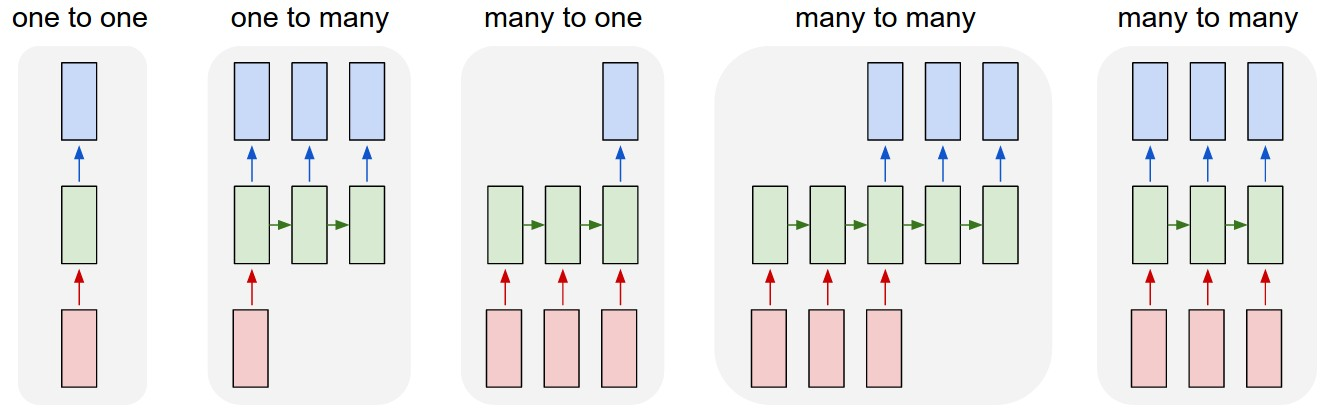
\includegraphics[width=100mm]{diagrams/rnn.jpeg}
	\caption{Rectangles represent vectors, with red being the input, blue the output, and green representing the state of the RNNs. Arrows represent  functions. From left to right: (1) an MLP. (2,3,4,5) are examples of different styles of recurrent neural networks, describing the different types of input and output combinations. (Diagram from \cite{karpathy_unreasonable_2015}) \label{rnn}} 
\end{figure}

At each time step $t$, a simple RNN produces a hidden vector $h_t$, derived from the input vector $x_t$ and the previous state $h_{t-1}$ in the function $h_t = f_w(h_{t-1}, x_t)$. The hidden vector is usually obtained by some affine transformation offset by a bias vector, described in more detail in equation \ref{eq:rnn}. The same function and the same parameters are used at each time step $t$. RNNs, by design, are not computationally parallelisable. This hidden vector $h_t$ is continously updated as it traverses through the RNN, learning the temporal relationships between the inputs.

\begin{figure}[!ht]
\begin{equation}
\label{eq:rnn}
\begin{aligned}
	h_t &= tanh(W_{hh}h_{t-1}+W_{xh}x_t)
\\
y_t &= W_{hy}h_t
\end{aligned}
\end{equation}
\captionsetup{labelformat=empty}
\caption{Equations for the RNN cell.}
\end{figure}

% talk about how they can be stacked.
RNN cells can be stacked, making a deeper recurrent network, and can also be bi-directional. Bi-directionality explores the temporal relationships of the sequence in both directions (left to right, and vice versa.) This is made possible by stacking two recurrent cells on top of each other, and having one forward propagate in one direction, and another in the opposing direction.

RNNs are typically trained with backpropagation through time (see equation \ref{eq:btt}) The gradient flow $w \leftarrow w - \alpha ({\delta L}/{\delta w})$ is computed at every timestep, meaning that every path from $W$ to the loss $\mathcal{L}$ needs to be considered.

\begin{equation}
\label{eq:btt}
\begin{aligned}
	\frac{\delta L}{\delta w} = \sum^T_{j=0}\sum^j_{k=1}\frac{\delta L_j}{\delta y_j}\frac{\delta y_j}{\delta h_j}(\prod^j_{t=k+1}\frac{\delta h_t}{\delta h_{t-1}})\frac{\delta h_k}{\delta w}
\end{aligned}
\end{equation}

Typically, there are two caveats with training RNNs. One of which involves the sensitivity of the gradients: The product symbol within the loss function in \ref{eq:btt} is the cause of vanishing and exploding gradients, both of which make it especially difficult to train RNNs. This is compounded by the fact that the limited expressibility of the gradients means that relationships between timesteps earlier in the recurrent computation are harder to train than timesteps further in the sequence. This is described as the long range dependency problem.

Additionally, it became aparrent that it was difficult for RNNs to establish relationships between potentially relevant non-contiguous inputs and outputs, especially in the case for longer sequences, there isn't necessarily a clear indicator in the architecture that would facilitate this feature. 

That being said, RNNs remains to be appropiate for language modelling primarily for its capability of encapsulating the temporally contextual relationships within the input sequence. The idea of recurrent language models can be realised in Section \ref{seq2seq}. Our paper revolves around the use of recurrent language models in a generative manner. We describe the generative capabilities further in Section \ref{variational_autoencoders}.

\subsection{LSTMs and GRUs} 

LSTMs and GRUs are types of recurrent cells, introduced to circumvent the issue of long range dependency problems, and gradient sentivities that RNN cells suffered.

% you should update the formulas
\begin{figure}[!ht]
\begin{equation}
  \begin{split}
    i_t &= \sigma(W_i \cdot [h_{t-1},x_t] + b_i) \\
    f_t &= \sigma(W_f \cdot [h_{t-1},x_t] + b_f) \\
		o_t &= \sigma(W_o \cdot [h_{t-1},x_t] + b_o) \\
		g_t &= \sigma(W_g \cdot [h_{t-1},x_t] + b_g) \\
		c_t &= f_t \odot c_{t-1} + i_t \odot g_t \\
		h_t &= o_t \odot tanh(c_t) 
  \end{split}
% \quad\leftrightarrow\quad
	\quad\quad
  \begin{split}
		u_t &= \sigma(W_u \cdot [h_{t-1},x_t] + b_u) \\
		r_t &= \sigma(W_r \cdot [h_{t-1},x_t] + b_r) \\
		c_t &= tanh(Ww_{t-1}+U(r_t \odot h_{t-1})) \\
		h_t &= (1-u_{t})\odot h_{t-1} + u_t \odot c_t
  \end{split}
\end{equation}
\caption{Equations for LSTM cells (left) and GRU cells (right).}
\end{figure}
 
LSTM (Long Short Term Memory; \cite{hochreiter_long_1997}) are a type of RNN cell that retains information based on the previous inputs through the introduction of gated architectures. These gated architectures regulate the flow of information coming to and from the cell, which helps to mitigate the issue of gradient sentivity and improves long range dependencies. Gates of the cell are parameterised and therefore learnable. LSTM cells can be swapped in place with the RNN cells. It has shown to have a considerably stronger performance for a variety of tasks compared to RNNs cells.

GRUs (Gated Recurrent Units; \cite{cho_properties_2014}) are functionally similar to LSTMs, but uses less parameters. Within the GRU architecture, a feature to retain the previous weights remain, but there exists an direct path to the input data from the output, allowing a reduction in training time. \cite{chung_empirical_2014} suggests that GRUs were found to perform at least equivalently to LSTMs but show slight improvements on smaller datasets. As there are objectively less parameters for the GRU, it should converge faster than LSTMs.

\section{Autoencoders}
\label{autoencoders}
% need citation
Autoencoders (\cite{e._rumelhart_learning_1986}) are a specialised form of neural networks where the model attempts to faithfully recreate the inputs on the output. This is made possible by learning the distribution of the input data. Autoencoders typically have a layer in the model where its dimension is smaller than the input space, therefore representing a dimensionality reduction in the data. Autoencoders can be considered to be a non-linear representation of PCA. Autoencoders within the domain of NLP are popularised through their use in Machine Translation, Word Embeddings, and document clustering. 

Autoencoders are composed of two different principal components, an encoder network $\alpha$ and a decoder network $\beta$, such that $\alpha : X \rightarrow F$ and $\beta : F \rightarrow X$. Note that $F$ is typically smaller in dimension than $X$, otherwise the model would be learning the identity vector.  Measuring the success of the reconstruction is deduced by a reconstruction loss formula. This reconstruction loss comapres the output of the decoder and compares it against the input of the encoder. The two networks are trained together in a manner that allows them to preserve the input as much as possible in the output.

% definitely need a diagram for autoencoders
% what is it good for?

% talk about how hard it is to understand the structure of the latent variable and how this prevents us from sampling.
Although the model learns the distribution of the data, unlike PCA one cannot immediately interpret the principal components of the data. In fact, it is difficult to understand the structure of the latent variable, as is the case for understanding the layers of neural networks in general. Additionally, as there is no sampling mechanism within this model, this effectively prohibits any generative capabilities. 

% talk about how important this is in the context of the task.
\subsection{Variational Autoencoders}
\label{variational_autoencoders}

% talk about how this can be a generative model.

Variational Autoencoders (VAEs, \cite{kingma_auto-encoding_2013}) stem away from regular autoencoders. As opposed to learning a fixed latent vector, VAEs force the encoder to learn parameters of a gaussian distribution - a mean $\mu$ and a covariance $\Sigma$. In more discrete terms, it replaces the encoder from the standard autoencoder with a learned posterior \textit{recognition model}, $q(z|x)$. This component of the autoencoder parameterises an approximate posterior distribution over $z$, using a neural network conditioned on $x$. This consequently allows us to take advantage of recent advances in variational inference.  A sample is taken from a gaussian using the learned parameters, which is then fed into the decoder. This sampling mechanism allows VAEs to have generative capabilities. For instance, one can entirely avoid the encoder network, and augment the mean and variance vectors to generate outputs from the decoder.

\begin{figure}[!ht]
	\centering
	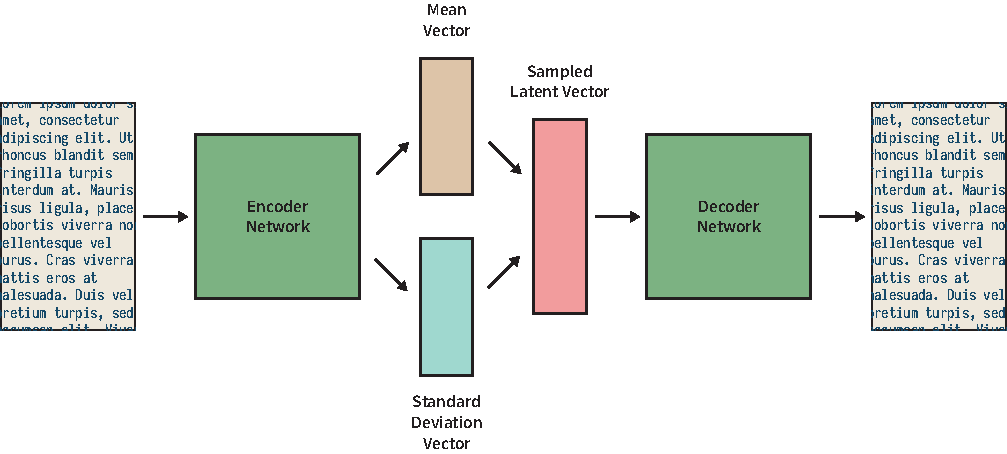
\includegraphics[width=150mm]{diagrams/variational_autoencoders.pdf}
	\caption{An abstracted model architecture for a variational autoencoder, which takes as input some text, and it's predicted output being the same text as the input.\label{vae}}
  \end{figure}

Note that the decoder receives samples from a non-standard normal distribution produced by the encoder. The average of the samples of the different distributions should approximate to a standard normal. This stochasticity allows us to model variability in the results. 

If VAEs were trained with a standard autoencoder's reconstruction objective, then it would learn to encode its inputs determinsitically by making variances in the \textit{recognition model}, $q(\overrightarrow{z}|x)$ vanishingly small. (\cite{raiko_techniques_2014}). When measured with KL Divergence, creates a obsolete value - This is known as a vanishing KL. (\cite{fu*_cyclical_2019}) Instead, the loss function for VAEs is composed of two components; a reconstruction loss that involves an expection of the output; and a KL divergence (see Equation \ref{eqn:kl_divergence}), which measures the distribution of the posterior distributions against a standard gaussian $ \mathcal{N}(0,1)$). This objective provides a tractable lowerbound on the true likelihood of the data, and forces the model to encode some information on the data into the gaussian parameters.
  
\begin{equation}
	\label{eqn:elbo}
	\mathcal{L}(\theta, \phi, x, z) = \mathbb{E}_{q \phi (z|x)}[log \thinspace p_{\theta}(x|z)] - D_{KL}(q_{\phi}(z|x)\thinspace||\thinspace p(z)) \leq log (p(x))
\end{equation}

\begin{equation}
	\label{eqn:kl_divergence}
D_{KL}(P ||Q) = \sum_{x \subset X} P(x) \cdot log (\frac{P(x)}{Q(x)})
\end{equation}

% In other words, it is the expectation of the logarithmic difference between the probabilities $P$ and $Q$, where the expectation of $P$ is already known.

\subsubsection*{Reparameterisation Trick}
\label{reparam_trick}
\begin{equation}
	z = \mathcal{N}(\mu, \Sigma) \equiv \mu + \Sigma \cdot \epsilon \\
	\label{eqn:reparam}
\end{equation}

Calculating gradients through backpropagation would be impossible as gradients would have to eventually push through a randomly sampled latent variable. The gaussian reparameterisation trick (\cite{kingma_auto-encoding_2013}) subverts this issue through the rearrangement of the gaussian parameters. Instead of sampling $z$ through a gaussian $\mathcal{N}(\mu, \Sigma)$, $z$ can be created rearranging the definition of the variable; a random sample through a gaussian can be redefined with a summation of $\mu$ and some gaussian noise $\epsilon \sim \mathcal{N}(0,1)$ applied to $\Sigma$. This rearrangement allows for derivatives to be calculated with respect to the parameters that are needed for learning as derivatives with respect to the relevant components would cancel out $\epsilon$.

\subsection{Conditional Variational Autoencoders}
\label{conditional_variational_autoencoders}
In a VAE, the decoder cannot produce outputs of a particular condition on demand. CVAEs add to the VAE to include conditioning on another description of the data, a class descriptor $y$. 

\begin{figure}[!ht]
	\centering
	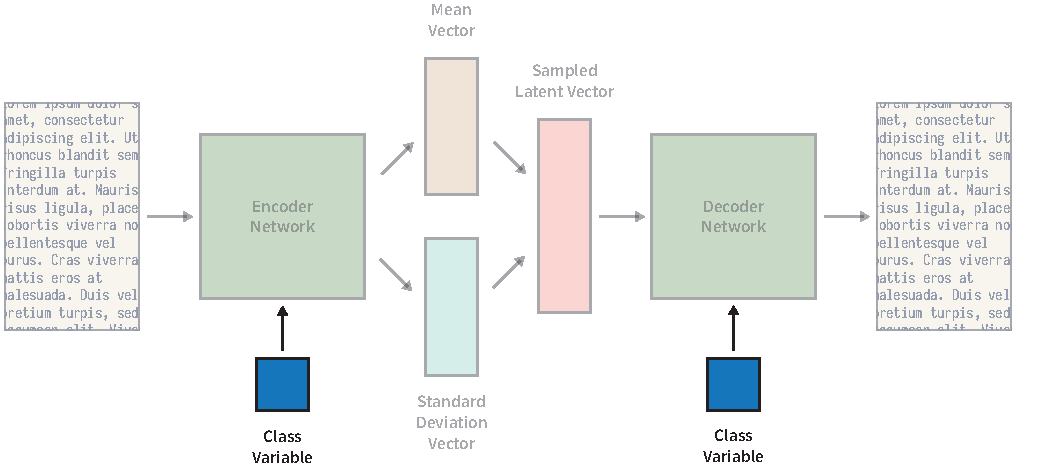
\includegraphics[width=150mm]{diagrams/conditional_variational_autoencoders.pdf}
	\caption{A model architecture for a CVAE, which includes the label being fed into the encoder and decoder networks. \label{cvae_diagram}}
\end{figure}

During training time, a class (represented by some arbitary vector) is fed at the same time to the encoder and decoder. To generate an output that depends on $y$ we feed that datum to the decoder along with a random point in the latent space sampled from a standard normal distribution.

Samples can be generated from the conditional distribution $p(x|y)$. By changing the value of $y$, we can get corresponding samples $x \sim p(x|y)$. The system no longer relies on the latent space to encode what output is necessary; instead the latent space encodes other information that can distinguish itself based on the differing $y$ values.

In terms of implementation, it happens to be more feasible to concate the class variable to the dataset prior to feeding. This allows the model to retain its characteristics without needing to adjust in order to accomadate the conditioning variables.

\section{Related Work}

% why?

\subsection{Sequence To Sequence}

Sequence to Sequence, (seq2seq, \cite{sutskever_sequence_2014}) is a type of neural language model that models relationships between sequences.  Seq2Seq comprises of two components, encoders and decoders (in a similar fashion to autoencoders), both of which are represented with RNN models (although as explained earlier, can be replaced with LSTM or GRU cells). The data it takes is a pair of sequential data, which for the example of text generation, would be query and response sequences. The query sequence would go through the encoder model. The last hidden state value of the encoder is used as the context variable, which encodes the characteristics of the input sequence. This is used as the first hidden vector value for the decoder, which would then predict the response sequence. 

% talk about how each word is fed into the input.

\begin{figure}[!ht]
		
\centering
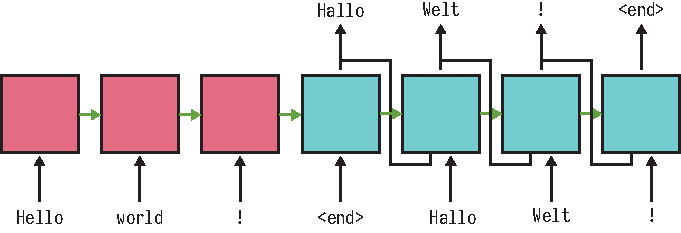
\includegraphics[width=100mm]{diagrams/seq2seq.pdf}
\caption{An abstracted model of the seq2seq architecture, where the encoder (pink) takes in the input sequence, and the decoder (blue) shows the output sequence. The encoder outputs are effectively ignored. \label{seq2seq}}
\end{figure}

Seq2seq models have shown to be effective in reponse generation, but is not without it's own set of problems. For instance, the context variable itself is considered to be the bottleneck as it has to encompass the properties of the entire input sequence in a single vector. As we've discussed earlier in Section \ref{rnn}, the training mechanism is subject to vanishing and exploding gradients, and that it becomes increasingly difficult to retain information about earlier parts of the sequence as opposed to recent parts of the sequence in the encoder stages as a consequence. We explain later about approaches to mitigate the issue.

Furthermore, the responses produced from a seq2seq model naturally lacks lexical diversity and richness (\cite{serban_hierarchical_2016}, \cite{zhao_learning_2017}, \cite{jiang_why_2018}). There tends to be many causes, but one reason (which we explore in the paper) is due to the lack of statistical inferencing. The model itself lacks the possibilty of presenting a variety of lexical responses in the decoder, in a manner that a VAE could.

\subsubsection{Variational Contextual Variables}
\label{variational_context}

\begin{figure}[!ht]
	\centering
	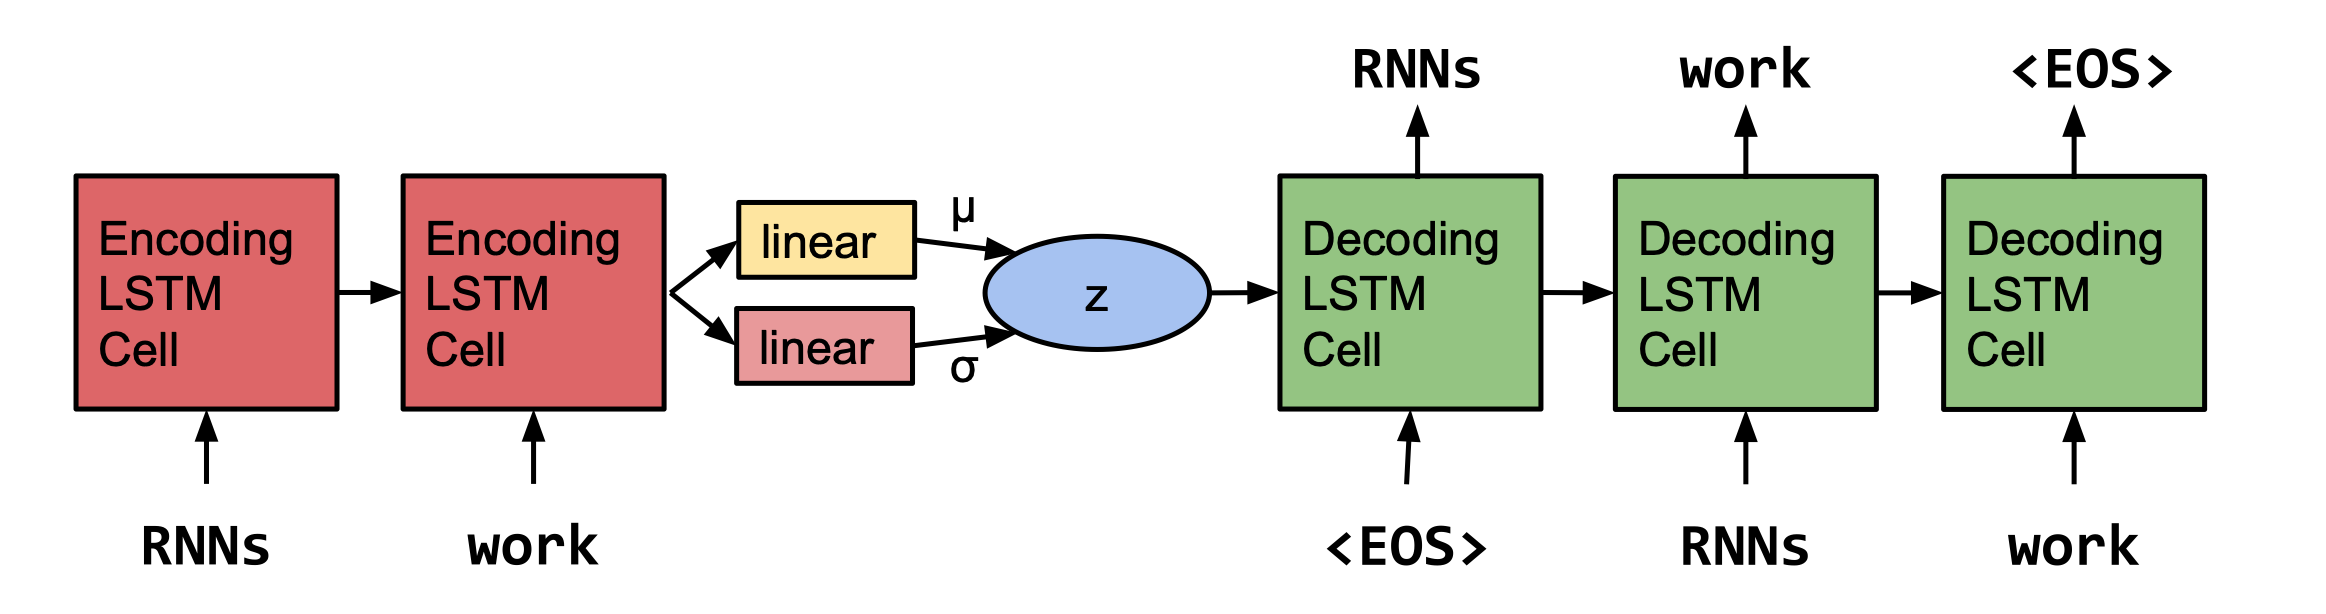
\includegraphics[width=100mm]{diagrams/seq2seqvae.png}
	\caption{The core structure of the VAE language model - words are represented as embedded vectors (\cite{bowman_generating_2015}). \label{vae_seq2seq}}
\end{figure}

Instead of passing through the last hidden state drom the encoder to the decoder, it is possible to encode the context variable produced from the encoder in the form of gaussian parameters in a similar fashion to how VAEs are designed (\cite{bowman_generating_2015}). The model is trained in a similar fashion to VAEs where the overall loss is composed of a reconstruction loss and a KL divergence (see Equation \ref{eqn:elbo}) but utilises additional mechanisms to force the language model to encode features into the gaussian parameters. We explain these features in further detail in Section \ref{optimisation_challenges}.

Although a neural language model based on this would be sufficient to generate responses, the responses would be generated from the same latent variable, restricting its variability in responses. (\cite{zhao_learning_2017};\cite{du_variational_2018})

\subsubsection{Attention Mechanism}

\begin{figure}[!ht]
      
	\centering
	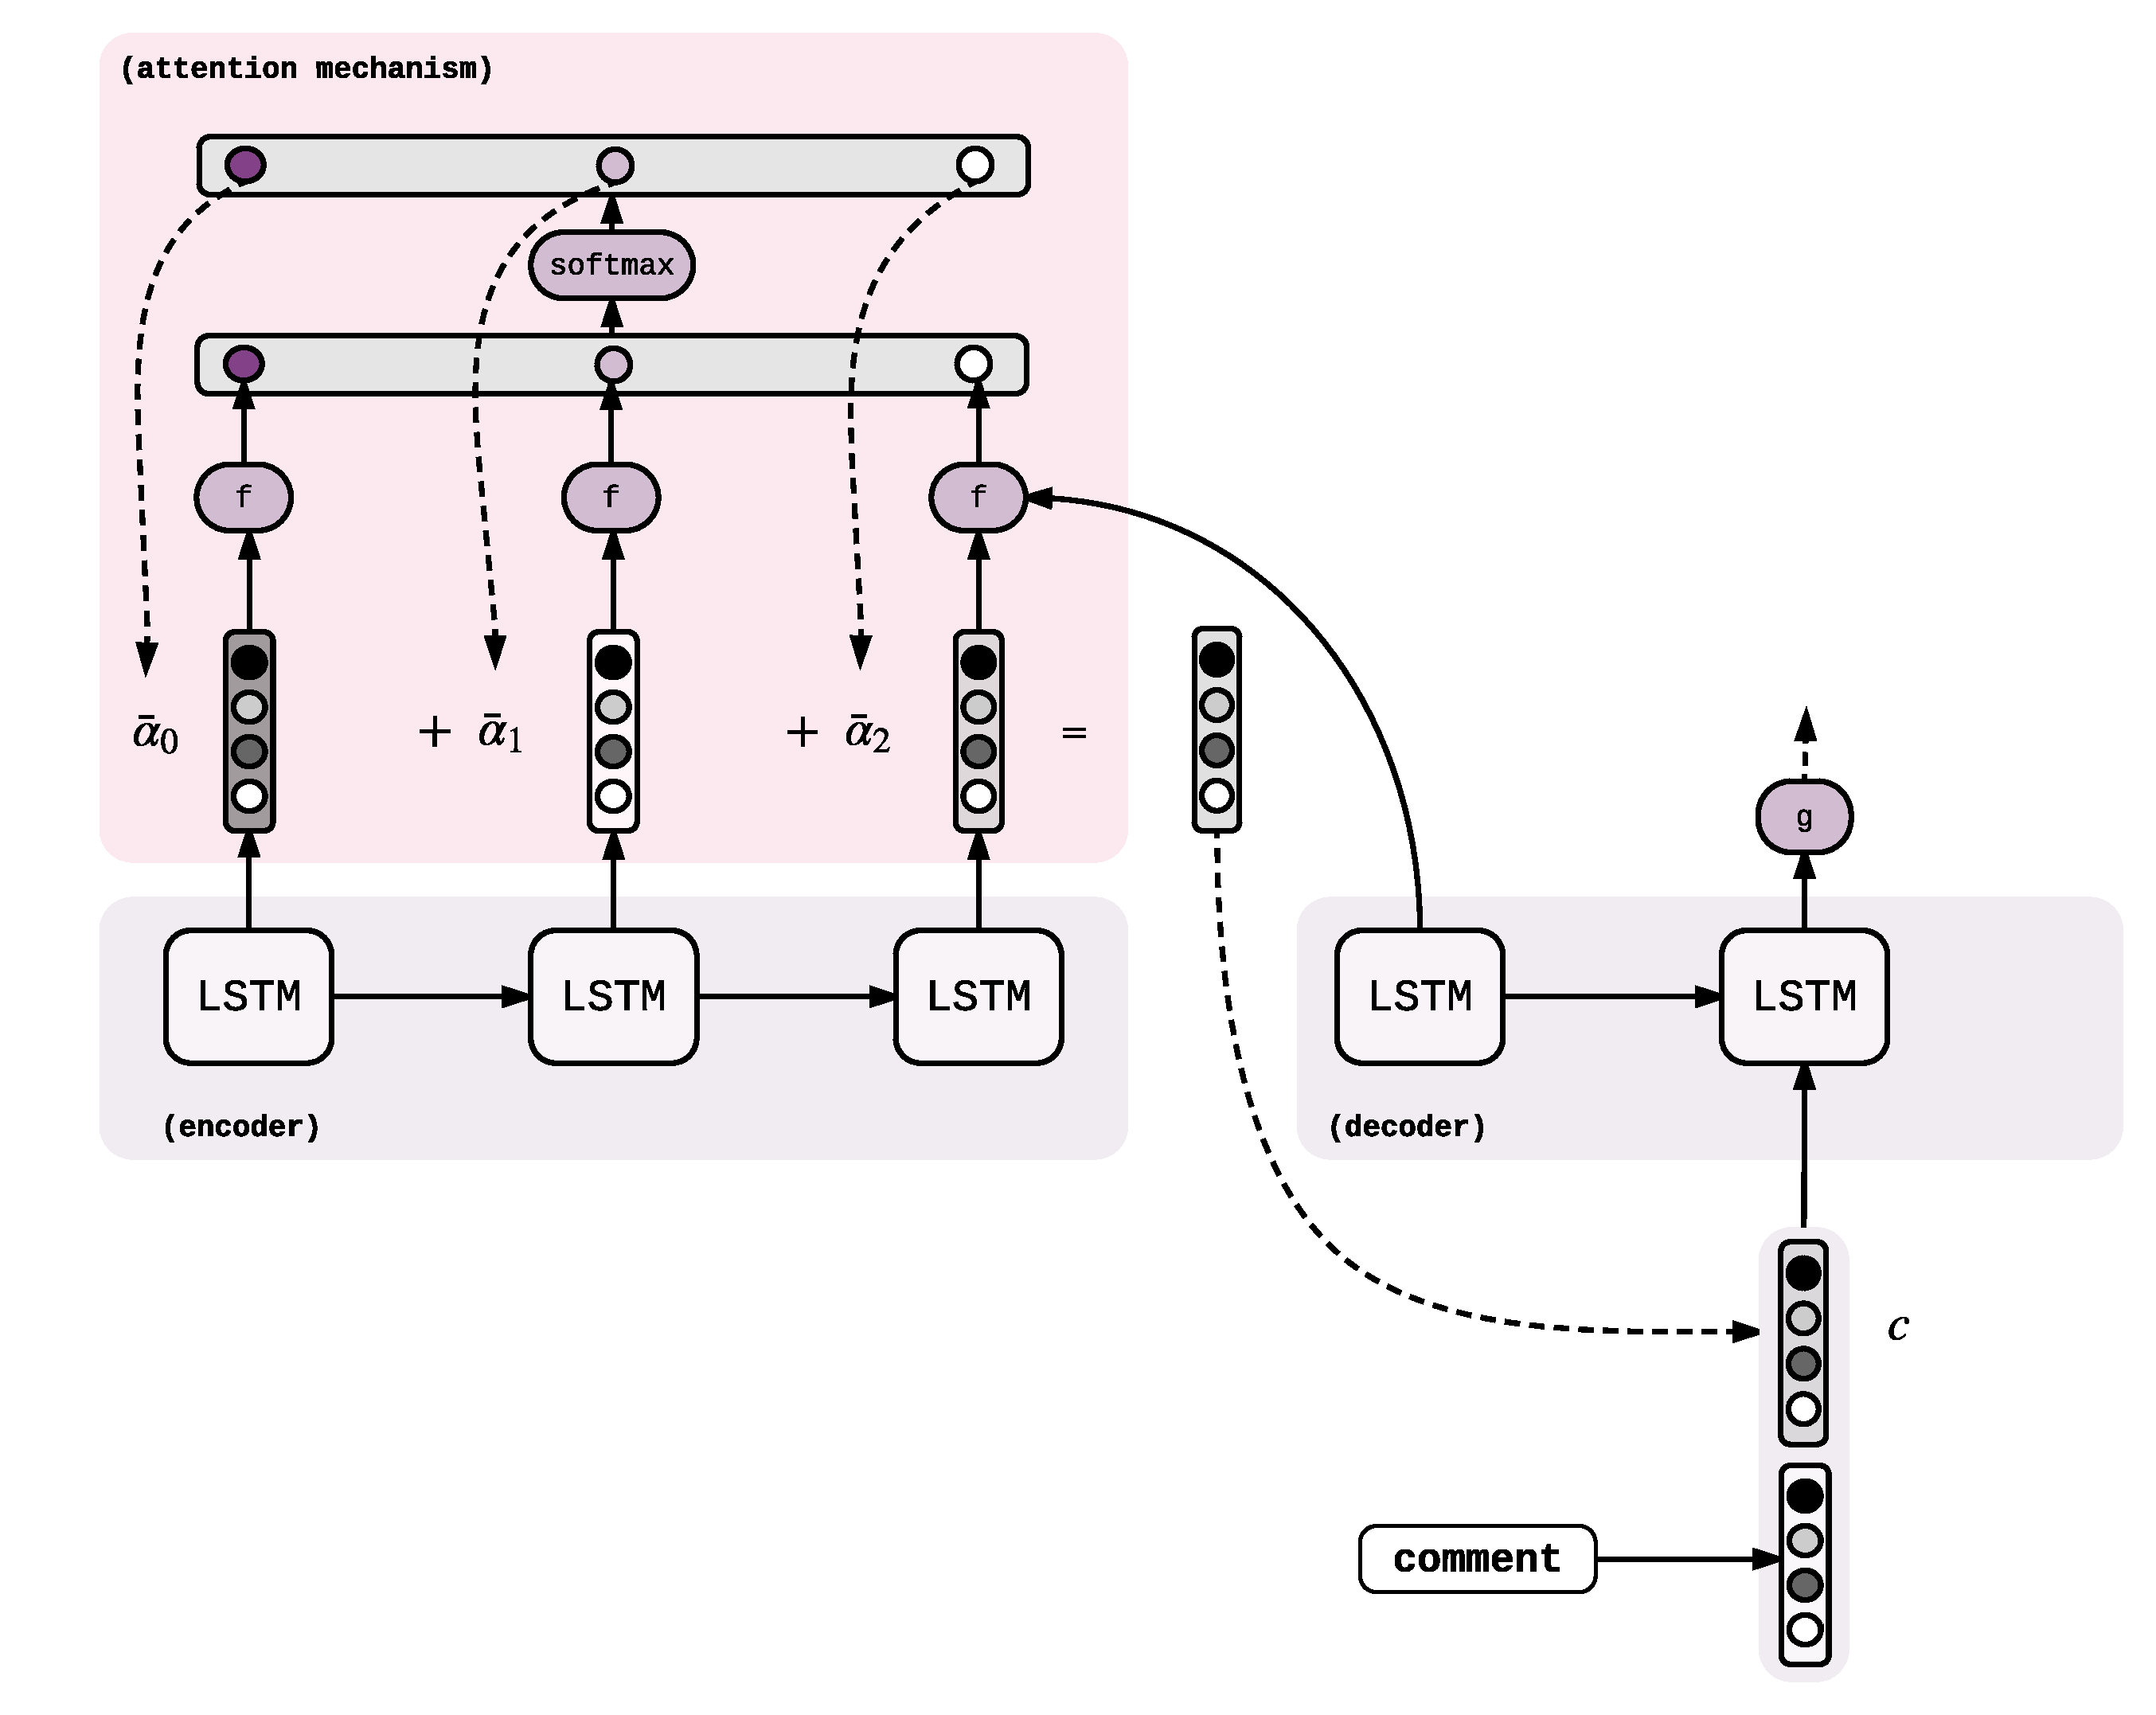
\includegraphics[width=100mm]{diagrams/seq2seq_attention_mechanism.pdf}
	\caption{An abstracted diagram of the attention mechanism, applied to a seq2seq model.\label{seq2seq_attn}}
\end{figure}
% https://guillaumegenthial.github.io/sequence-to-sequence.html

In addition to the context vector, the decoder can also retrieve non-contiguous relationships on the encoder values using attention (\cite{bahdanau_neural_2014}). This mechanism looks at all of the inputs from the hidden states of the encoders so far. This allows the decoder network to "attend" to different parts of the source input at each step of the output generation. This would work in tandom with the context vector provided from the encoder, helping the model with long-range dependency problems.

Furthermore, this attention mechanism allows the model to learn what to attend to based on the input sequence and what it has so far, represented through a weighted combination of the two.

Attention mechanisms were found to perform particularly well in machine translation problems where languages which are relatively well aligned (such as English and German). The decoder is most likely able to choose to attend to the response generation sequentially, such that the first output from the decoder can be generated based on the properties of the first input of the encoder and so on.

\subsection{CVAE Seq2Seq}

To increase variability of outcomes produced by the original VAE seq2seq model, \cite{zhao_learning_2017} adapted the original implementation by \cite{bowman_generating_2015} for the purposes of discourse generation. It includes a plethora of additional components, including attention mechanisms to make discourse generation more viable.

\subsubsection{Bayesian Modelling}

\subsubsection{Knowledge Guidance}
Sequences are conditioned by their dialog act, and a utterance encoder. 

\subsubsection{BOW Loss}
One of the novel approaches the model has suggested was the inclusion of a BOW loss. 

Although this introduces variability in the outputs, the variability is not controlled; i.e it is produced from the randomness of $z$. The underlying seq2seq model remains suboptimal.

\chapter{Model}

% mention the limitations of Seq2seq for your problem and ways they could be addressed (VAEs, etc.), describe the VAE approach and your motivation to pick it, introduce the VAE paper you work with in details.

In this chapter we discuss the variational autoregressive decoder (VAD) in detail. It builds on the knowledge found in the literature review, and the model itself is a combination of the components and models described above. To help fully understand the capabilities of the VAD, we subject it to a series of datasets to understand how it works and its performance against them. The VAD has been shown to encapsulate a distribution of the data within the latent parameters well compared to the CVAE Seq2Seq (\cite{zhao_learning_2017}), and retains a high KL ratio respective to its overall loss function. This could potentially be used as the primary mechanism for encapsulating models, which can be sent to clients as a means of solving our case scenario.

\section{Variational Autoregressive Decoders}

Introduced by \cite{du_variational_2018}, VADs attempt to circumvent the sampling problem introduced from CVAEs by introducing multiple latent variables into the autoregressive Decoder. At different time-steps, this allows the decoder to produce a multimodal distribution of text sequences, allowing a greater variety of responses to be produced. 

\begin{figure}[!ht]
		
	\centering
	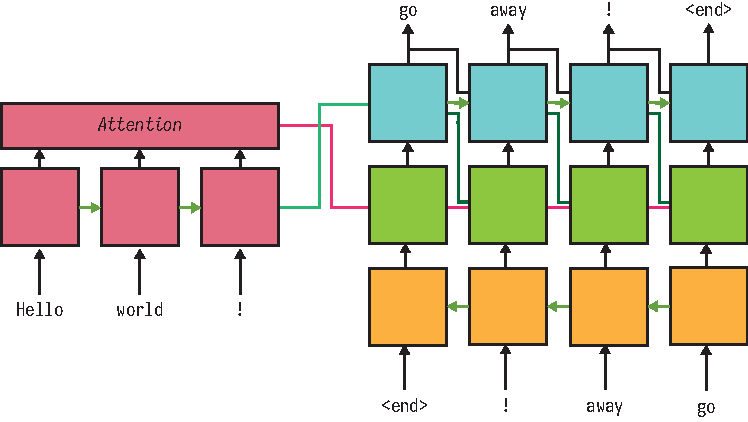
\includegraphics[width=100mm]{diagrams/vad.pdf}
	\caption{An abstracted model of the VAD model, where the encoder (pink) takes in the input sequence, orange represents the backwards model, green represents the latent, context generation, and the decoder (blue) shows the output sequence.\label{vad_abstract}}
	\end{figure}

VADs use the vanilla seq2seq architecture as the base (Section \ref{seq2seq}) with variable-length queries $x = \{x_1, x_2, ..., x_n\}$, and $y = \{y_1, y_2, ..., y_n\}$ representing the query and response sequences respectively. Both the encoder and decoder utilises GRUs, with the encoder utilising a bidirectional GRU, and the decoder being unidirectional. For each timestep $t$, each GRU in the decoder network is encoded with hidden state $h^d_t$. The components of the model are broken down into their subsections below.

% need a diagram

\subsubsection{Encoder}

\begin{align}
\label{eqn:eqlabel}
\begin{split}
	\overrightarrow{h^e_t} = \overrightarrow{GRU}(x_t, \overrightarrow{h^e_{t-1}})
\\
\overleftarrow{h^e_t} = \overleftarrow{GRU}(x_t, \overleftarrow{h^e_{t+1}})
\end{split}
\end{align}

The encoder works in a similar fashion to the encoder described in the seq2seq network. The only changes here we see is that the encoder described in the implementation leverages bi-directionality. Similarly to the seq2seq and other recurrent language models, the last hidden vector is passed through as the initial hidden vector for the decoder model.

\subsubsection{Backwards and Attention}


% you should update the formulas
\begin{figure}[!ht]
	\label{eqn:eqback}
	\begin{equation}
		\begin{split}
			\overleftarrow{h^d_t} &= \overleftarrow{GRU}(y_{t+1}, \overleftarrow{h^d_{t+1}})
			% i_t &= \sigma(W_i \cdot [h_{t-1},x_t] + b_i) \\
			% f_t &= \sigma(W_f \cdot [h_{t-1},x_t] + b_f) \\
			% o_t &= \sigma(W_o \cdot [h_{t-1},x_t] + b_o) \\
			% g_t &= \sigma(W_g \cdot [h_{t-1},x_t] + b_g) \\
			% c_t &= f_t \odot c_{t-1} + i_t \odot g_t \\
			% h_t &= o_t \odot tanh(c_t) 
		\end{split}
	% \quad\leftrightarrow\quad
		\quad\quad
		\begin{split}
			\alpha_{s,t} &= f_{attention}([h^e_d, h^d_{t-1}]) \\
			c_t &= \sum^m_{s=1}\alpha_{s,t} h^e_s
			% u_t &= \sigma(W_u \cdot [h_{t-1},x_t] + b_u) \\
			% r_t &= \sigma(W_r \cdot [h_{t-1},x_t] + b_r) \\
			% c_t &= tanh(Ww_{t-1}+U(r_t \odot h_{t-1})) \\
			% h_t &= (1-u_{t})\odot h_{t-1} + u_t \odot c_t
		\end{split}
	\end{equation}
	\caption{Equations for Backwards (left) and Attention (right).}
	\end{figure}


The backwards RNN is used to feed additional contextual information for the inference model.  During training, the backwards RNN takes as input the training outputs $y$ and outputs hidden vectors in a reverse, sequential manner. The VAD leverages the attention mechanism in a similar manner, and takes in the input sequence, and is contextualised by the decoder at a given timestep.

\subsubsection{Inference and Prior Models}

\begin{figure}[!ht]
	\label{eqn:inf_prior}
	\begin{equation}
		\begin{split}
			\lbrack \mu^i, \sigma^i \rbrack &=
			f_{infer}([\overrightarrow{h^d_{t-1}}, c_t, \overleftarrow{h^d_t}])
			\\
			q_{\theta}(z_t|\boldsymbol{y}, \boldsymbol{x}) &= \mathcal{N}(\mu^i, \sigma^i)
		\end{split}
	% \quad\leftrightarrow\quad
		\quad\quad
		\begin{split}
			\lbrack \mu^p, \sigma^p \rbrack &=
			f_{prior}([\overrightarrow{h^d_{t-1}}, c_t])
			\\
			p_{\phi}(z_t|\boldsymbol{y}_{<t}, \boldsymbol{x}) &= \mathcal{N}(\mu^p, \sigma^p)
		\end{split}
	\end{equation}
	\caption{Equations for Inference (left) and Prior (right) models.}
	\end{figure}

The inference model attempts to learn a conditional posterior distribution $z$ using the output, the attention weights, and the decoder outputs. $z$ is created using the gaussian reparameterisation trick described in Section \ref{reparam_trick}.

This component stems away from \cite{zhao_learning_2017}, as $\boldsymbol{z}$ is now decomposed into sequential variables $\boldsymbol{z} = \{z_1,...,z_t\}$, which are generated at each time step of the decoder phase. $z_t$ is conditioned by the backwards hidden vector $h^d_{t}$. \cite{du_variational_2018} suggests that this conditioning allows the latent variables to be guided for long-term generation.

The prior network is restricted to using observable variables during testing of the model to generate $z_t$ using only observable data. It is designed in a similar fashion to the decoder network where the input variables are concatenated together. Note that the prior is no longer a standard gaussian; this particular component would learn to approximate the posterior distribution.

\subsubsection{Decoder (Variational Autoregressive)}

\begin{equation}
	\begin{split}
		\overrightarrow{h^d_t} &= \overrightarrow{GRU}([y_{t-1},c_t,z_t], \overrightarrow{h^d_{t-1}}) \\
		p_\phi(y|\boldsymbol{y}_{<t},\boldsymbol{z}_t, \boldsymbol{x}) &= f_{output}([\overrightarrow{h^d_t}, c_t])
	\end{split}
\end{equation}

The decoder then takes in the temporally conditioned $z_t$, alongside the previous output $y_{t-1}$ and the context vector produced from the attention mechanism $c_t$ to produce the output.

\subsubsection{Auxillary Objective}

One of the novel contributions of the model is the use of a temporally contextual auxiliary objective that uses the sampled latent vector $z_t$ to predict the sequential bag of words (SBOW) of the response sequences $\boldsymbol{y}_{bow}(t+1,T)$. Let $f=MLP_b(z_t) \in \mathcal{R}^V$ where $V$ be the vocabulary size, then the bag of words can be deduced using the following equation:

\begin{equation}
	log [p_\xi(y_{bow(t+1,T)}|z_{t:T}) ] = log  \frac{e^{f_{z_{t}}}}{\sum^V_j e^{f_{j}}}
\end{equation}

The intuition is that this auxiliary objective would help to improve the KL divergence, as the latent variables would capture the information from a different perspective (\cite{du_variational_2018}).

\subsubsection{Learning Mechanism}


VADs uses the ELBO (Equation \ref{eqn:elbo})\footnote{As the KL divergence no longer compares the latent variable against a standard gaussian, we derive the equation to allow gradient propagation between two arbitary distribution. This can be seen in the Appendix (Section \ref{kl_derivation}).} and a weighted log likelihood loss of the auxillary objective, controlled by $\alpha$. This loss is computed at each timestep, and is then summed at the end of the sequence generation during the decoder stage. During training and evaluation, we sample both the inference and prior models to facilitate measuring the loss. The KL divergence allows the model to perform discourse generation using the prior mdoel.

\begin{equation}
	\begin{split}
		\mathcal{L} &= \sum_t [\mathcal{L}_{ELBO}(t) + \alpha \mathcal{L}_{AUX}(t)] \\
		\mathcal{L} &= \sum_t [(\mathcal{L}_{LL}(t) - \mathcal{L}_{KL}(t)) + \alpha \mathcal{L}_{AUX}(t)] 
	\end{split}
\end{equation}

During implementation, it was found that the auxiliary loss weight $\alpha$ typically initially increases the KL divergence, but eventually produces a diminishing effect to both the auxiliary loss and the KL divergence. Attempts to contact the original authors of the VAD paper were to no avail, and is left for future work. 

% Although these models have been used in NMT related problems, sequence generation is often unexplored within NLP. We propose using models that traditionally perform well in NMT problems and adapt them for use with sequence generation problems. 


\section{Optimisation Challenges}
\label{optimisation_challenges}

In addition to the fact that RNNs itself are difficult to train (see Section \ref{rnn}), it is often the case that the latent variable is often ignored during training. Ideally, a model that encodes useful information in the latent variable $\overrightarrow{z}$ will have a non-zero KL divergence term and in addition to a relatively small cross-entropy term. Straightforward implementations of our model failed to learn this behaviour.

Due to the sensitivity of the latent component, which is compounded by the sensitivity of the recurrent cells in the VAD, early builds of the VAD would often ignore $\overrightarrow{z}$ and go after the low hanging fruit during the learning process of the decoder. Once this occurs, the decoder ignores the encoder and gradients between the two components become non-existent, inhibiting learning on the gaussian parameters.

is it often likely that in a degenerative setting, the latent vector in the model would encorporate a lack of relevant information and is essentially ignored. This results in a KL collapse such that the KL loss reaches zero, and thus the model is then effectively equivalent to an RNN language model. Alongside the SBOW discussed earlier, we discuss other approaches to overcome any learning difficulties.

\subsection{Teacher Forcing}

Teacher Forcing (\cite{williams_learning_1989}) is a concept of using real target outputs as each next input in the decoder sequence as opposed to using the decoder's guess. This causes the model to converge faster, but may exhibit instability when the trained network is exploited. Typically, this can be controlled with a probability $p$ such that the decoder sequence has a $p$ chance of using teacher forcing during training.

Outputs can be observed when using teacher forced decoders that read with coherent grammar, but the generated response can wander far from the correct response; i.e. with some $p<1$, some outputs from the decoder at some timestep would be correct, but the others would have a chance to completely change the semantics of the output. We initially set $p=1$, but we set $p$ to be explored during the hyperparameter search.

\subsection{KL Annealing}

A simple approach by \cite{bowman_generating_2015}, it involves adding a variable weight to the KL term in the cost function at training time. Initially, the weight is zero, forcing the model to encode as much information into the latent variable as much as it can. The weight is then gradually increased, eventually reaching 1. At this stage the weighted cost function is equivalent to the ELBO loss. This could be thought of as annealing from a regular autoencoder towards a variational one.

That being said, Bowman et al. exposes a variety of additional hyperparameters including the step size, the total number of steps, the step rate (for instance, a linear progression or a logistic). For the sake of simplicity, we explore a linear approach with a fixed linear progression.

\subsection{Word Dropout}
Also proposed by \cite{bowman_generating_2015}, it involves weakening the decoder by removing some conditioning information during training. This is done by randomly replacing a fraction of the conditioned-on word tokens with a generic unknown token UNK, which forces the model to depend on the latent variable $z$ for prediction. This works in a similar fashion to the standard dropout (\cite{srivastava_dropout:_2014}) where connections are dropped between layers of a network, but is applied to the input data of a recurrent cell. We do not explore this technique further for the VAD as other reports indicate it's distruptiveness and that it was also not considered in the original VAD paper.

\chapter{Experimental Setup}

We compare three neural language models: a baseline model, a VAE Seq2seq (see Section \ref{variational_context}) and the VAD model. the baseline model represents a encoder-decoder seq2seq network (\cite{serban_hierarchical_2016}) that uses the same architecture base as the VAD but only minimises the standard cross entropy loss (i.e. the BOW loss and KL divergence computations are not computed). We use this approach instead of using a different implementation as it was acknowledged earlier in the paper that a KL collapse on variational sequential models is effectively equivalent to a RNN language model. 

For all intents, the VAE Seq2Seq model is primarily designed for language modelling, whereas the VAD is designed for dialog response generation. With this prior knowledge we expect the VAE Seq2seq model to perform worse than the VAD model for all tasks.

The seq2seq model and the VAE Seq2seq models were chosen for comparision not necesssarily to compare state-of-the-art performance but to verify the correctness of the implementations against our VAD model. We do not implement the CVAE seq2seq model as it is not the focus of the ISO.

\subsection*{Weight Initialisation}

Typically, we intend to have the weights asymmetricly generated (such that when we perform our gradient descent we would have random starting positions, which would enable us to have a better chance to find the minimum as opposed to having a fixed starting point).

\cite{glorot_understanding_2010} proposed to initialise the weights based on a gaussian $Var(w)=\mathcal{N}(0,\frac{2}{|n_{in}| + |n_{out}| })$ where $w$ represents a layer in a network, and $|n_{in}|$ represents the number of neurons feeding into it, and similarly so for $|n_{out}|$. Note that I have used a gaussian distribution, but it can also be uniform. This method has shown a lot of success for sigmoidal and tanh based activation functions. We initialise all weights with this method for their default values.

\section{Datasets}

We subject the models to three different datasets: Amazon Reviews (\cite{he_ups_2016}), Penn TreeBank (\cite{marcus_building_2002}), and OpenSubtitles (\cite{lison_opensubtitles2016:_2016}). Each dataset serves a different purpose; we describe them in their respective sections.

\subsection{Amazon Reviews}

\begin{figure}[!ht]
	\centering
	\lstinputlisting[language=java]{dataset_amazon_1.txt}
	\lstinputlisting[language=python]{dataset_amazon_2.txt}
	\caption{A sample review and the augmented data. Note that for each sequence from line 3 onwards has the identity sequence contatenated before it. \label{aug_1}}
\end{figure}

The Amazon products reviews (\cite{he_ups_2016}) comprises a set of customer submitted reviews of products on the popular consumer commerce website Amazon.com, spanning May 1996 - July 2014. For the purposes of this ISO, we select the electronic products dataset, spanning 1.6m reviews, but due to computational constraints, we work on a subset of this dataset as reviews would also need to be broken down into sequences of sentences. This dataset is used as the primary indicator of the performance of the models in their capability for text generation.

The model would be forced to produce the next sentence from the previous sentence. Sentences are split by periods. Tokens are represented as words or individual punctuation marks. Additional tags are introduced. Lowercase. The product is represnted by an ASIN, which effectively represents the item ID. this is split by characters.
% talk about tokenisation with SpaCy

Pre-processing includes (1) sentenissation and tokenisation using SpaCy (\cite{honnibal_spacy_2017}); (2) concatenation of sequence conditioning on the input sequences; (3) keeping the top 10K frequent word types af the vocabulary; (4) removing sequences where the "<unk>" tags in the sequences represent a ratio of greater than 0.1; (5), and finally removing sequences that are greater than a length of 60. 

% use GloVe Word embeddings

GloVe Word embeddings (\cite{pennington_glove:_2014}) are used to represent tokens in the dataset, and is also used to determine words to remove. 

For some conditional tags, we augment 
We compute discrete polarity value $p$ with a rounded ratio $p=round(r_{+}/r_{-},2)$. The polarity word vector is a sum of the polarity value $p$ and the word vector corresponding to the word "polarity".

% talk about conditioning on the sequences

We intend to augment the dataset such that the sequences are conditioned by the item ID, rating, and polarity of the review.

% talk about the distribution of the sequence lengths and unk words

\subsection{OpenSubtitles}

\begin{figure}[!ht]
	\centering
	\lstinputlisting[language=java]{dataset_opensubs_1.txt}
	\lstinputlisting[language=java]{dataset_opensubs_2.txt}
	\caption{A sample review and the augmented data. Note that for each sequence from line 3 onwards has the identity sequence contatenated before it. \label{aug_1}}
	\end{figure}

Additionally, we use OpenSubtitles. They are setup in a similar fashion to how the amazon dataset is setup, but does not involve conditioning. GloVe is also used. This particular dataset was used as one of the benchmark examples in the VAD model (\cite{du_variational_2018}) and is primarily used to compare disparity of the results between ours and the proposed VAD model in their paper.

In a similar fashion to the Amazon electronics dataset, pre-processing includes (1) sentenisation and tokenisation using SpaCy (\cite{honnibal_spacy_2017}); (2) concatenation of sequence conditioning on the input sequences; (3) keeping the top 10K frequent word types af the vocabulary; (4) removing sequences where the "<unk>" tags in the sequences represent a ratio of greater than 0.1; (5), and finally removing sequences that are greater than a length of 60. 

% talk about the distribution of the sequence lengths and unk words

\subsection{Penn TreeBank}

% No word embeddings
% no conditioning
% preformatted

\begin{figure}[!ht]
	\centering
	\lstinputlisting[language=java]{dataset_penn.txt}
	\caption{A sample review and the augmented data. Note that for each sequence from line 3 onwards has the identity sequence contatenated before it. \label{ptb_example}}
	\end{figure}

For quick configuration with the model, we compute initial results with the Penn Tree-Bank Dataset. (\cite{marcus_building_2002}) This dataset is typically used for verification of model performance for generative models; the dataset consists of sequences which are the same for the input and output. (See \ref{ptb_example}) For the purposes of the ISO, we used the exemplar dataset which consists of 43K sequences. Pre-processing includes (1) tokenisation using NLTK; (2) trimming sequences that are greater than a length of 60; (3) replacing tokens with <unk> where the token does not exist in the vocabulary. For this particular dataset, we do not use any pre-trained word-embeddings; as the intention of the dataset does not benefit from its addition. 

% talk about how it's conditioned.



\section{Hyperparameter Setup}

For the sake of comparisons, all models leverage a bidirectional encoder. For variational models we utilise a linear KL annealing with a step size of $2.5\cdot 10^{-5}$ with a threshold of 2000 steps. Dimension sizes for the hidden sizes are 512, with latent sizes being 400, and are not hyperparameterised. The cross entropy loss, KL loss, and BOW losses are normalised by the sequence length. 

All models use the Adam optimiser (\cite{kingma_adam:_2014}) with a base learning rate of 0.001; subject to hyperparameterisation. Models are computed on a linux machine with a  4.4GHz intel 3770k CPU with a GTX 1080 GPU with 8GB VRAM, and 32GB RAM.

As we measure the performance of three fundamentally different neural language architectures, we performed hyperparameter tuning for each of the models independently.

Datasets were split in a 80:15:5 ratio, for training, validation, and test data respectively. Models were subject to roughly 15 hyperparameter tuning rounds (dependent on the confidence of the optimisation model) using Bayesian Optimisation (\cite{gpyopt_authors_gpyopt:_2016}) where the objective is to minimise the loss. Early stopping is initialised such that the training will end when the mean loss of the validation batch is reached. 

\section{Measuring Performance}


\subsection{BLEU and ROUGE}

Talk about it being infeasible to cherrypick responses used for classification so we take the mean output and comptue bleu and rouge.

To understand the quality of our models, we subject them to the BLEU (\cite{papineni_bleu:_2001}) and ROUGE (\cite{lin_rouge:_2004}) emperical scores at each epoch to quantify the quality of our responses. These measurements are used alongside the Loss, and human analysis of the results.

BLEU (\cite{papineni_bleu:_2001}) is originally defined with $n$-gram precision $p_n$ by summing the $n$-gram matches for every hypothesis sentence $S$ in the test corpus $C$. In our particular case, we use unigrams.

\begin{figure}[!ht]
	\begin{equation}
		\begin{split}
			p_n = \frac
			{\sum_{S\in C} \sum_{ngram\in S} Count_{clip}(ngram)}
			{\sum_{S\in C} \sum_{ngram\in S} Count(ngram)}
		\end{split}
	% \quad\leftrightarrow\quad
		\quad\quad
		\begin{split}
			p_n = \frac
			{\sum_{S\in C} \sum_{ngram\in S} Count_{matched}(ngram)}
			{\sum_{S\in C} \sum_{ngram\in S} Count(ngram)}
		\end{split}
	\end{equation}
	\caption{Equations for BLEU (left) and ROUGE (right).}
	\end{figure}

% https://stackoverflow.com/questions/38045290/text-summarization-evaluation-bleu-vs-rouge

Although both equations look very similar, BLEU introduces a brevity penalty term, and also compute the n-gram match for several sizes of n-grams (unlike the ROUGE-n, where there is only one chosen n-gram size). 

Additionally, we use BLEU to measure the precision performance, i.e. how much the words (and/or n-grams) in the model responses appeared in the responses from the dataset. ROUGE is used in a similar fashion for recall.

Naturally - these results are complementing, as is often the case in precision vs recall. If you have many words from the system results appearing in the human references you will have high Bleu, and if you have many words from the human references appearing in the system results you will have high Rouge."

\begin{figure}[!ht]
	\begin{equation}
		f1_{1} = 2 \frac{BLEU_1 \cdot ROUGE_1}{BLEU_1 + ROUGE_1}
	\end{equation}
	\caption{The harmonic mean of BLEU and ROUGE scores.}
\end{figure}

To understand an overall picture of the model performance, we also measure the harmonic mean of BLEU and ROUGE, by considering the F1 performance. We consider that the larger the F1 performance, the more faithful the model is in replicating the sequences of the output data given its conditioning.

\chapter{Experimental Results}
% http://opennmt.net OPENMNT-Py has BLEU/ROUGE on it.

% %%%%%%%%%%%%%%%%%%%%%%%%%%%%%%%%%%%%

\section{NLL Loss}

\begin{figure}[!ht]
	\centering
	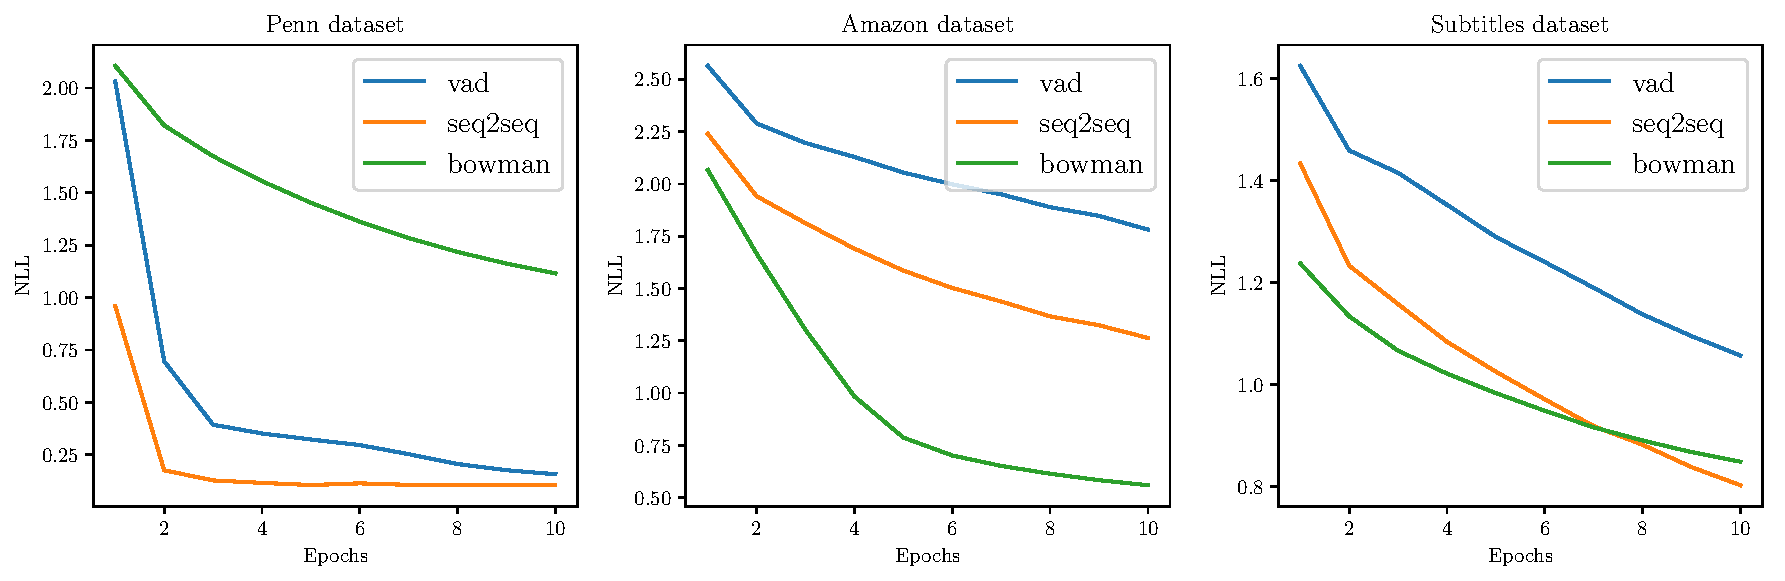
\includegraphics[width=150mm]{results/nll.pdf}
	\caption{Reconstruction losses of the three models across the three datasets; lower loss is better. \label{r:nll}}
  \end{figure}

% what is it? how is it measured? what does it say
The results shown are not necessarily surprising. As there are less weights to learn, it was expected as the vanilla seq2seq model to converge faster than the other models. Conversely, it was expected for the VAD model to converge the slowest considering the number of weights involved.

Additionally, varational models are expected to perform worse than discrete models as they leverage an entirely different training mechanism; learning parameters of a gaussian is also hard to condition (see the next section for more information).
% talk about the fact that this is not a good start anyway

\section{KL Loss}

\begin{figure}[!ht]
	\centering
	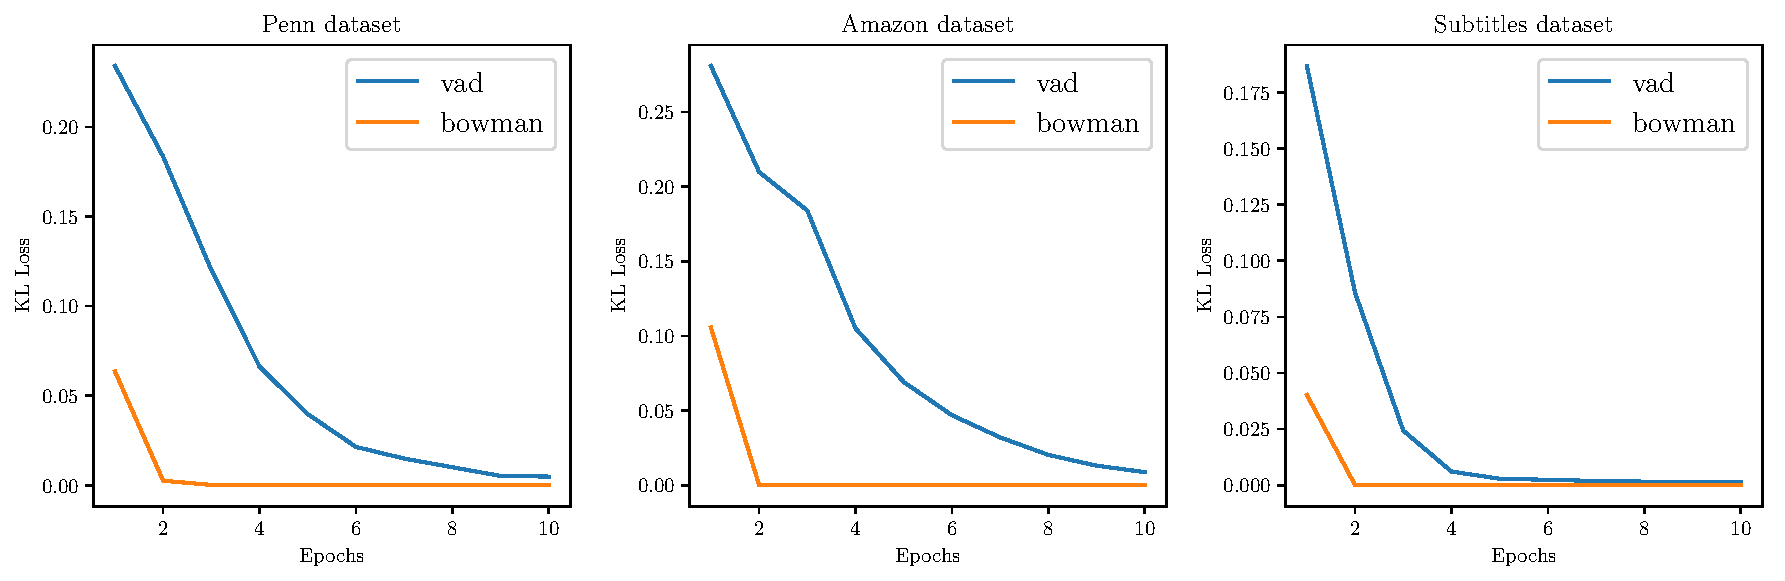
\includegraphics[width=150mm]{results/kl_loss.pdf}
	\caption{KL losses of the three models across the three datasets; higher is better.\label{r:kl_loss}}
	\end{figure}
	
We measure the KL loss to determine the rate of which the KL 

% talk about KL collapse
% what is it? how is it measured? what does it say

\section{KL Ratio}

\begin{figure}[!ht]
	\centering
	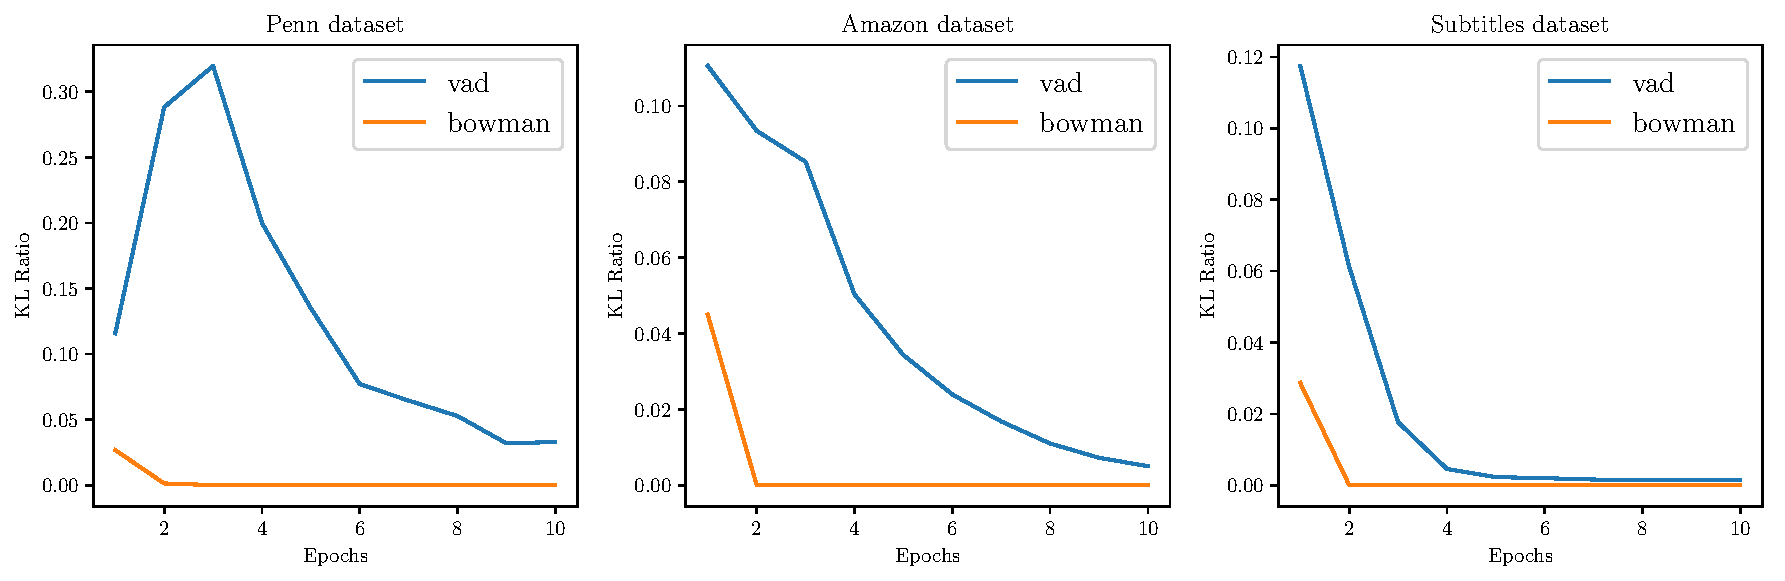
\includegraphics[width=150mm]{results/kl_ratio.pdf}
	\caption{KL ratios of the three models across the three datasets; higher is better.\label{r:kl_ratio}}
  \end{figure}

The intent of measuring the KL Ratio is such that we would be able to see a good picture of how much information was encompassed in the latent variable, and thus retaining more characteristics of the variational autoencoder as opposed to a regular autoencoder. 
Interestingly, we can see KL collapse with the 

% what is it? how is it measured? what does it say

\section{BLEU and Rouge}

\begin{figure}[!ht]
	\centering
	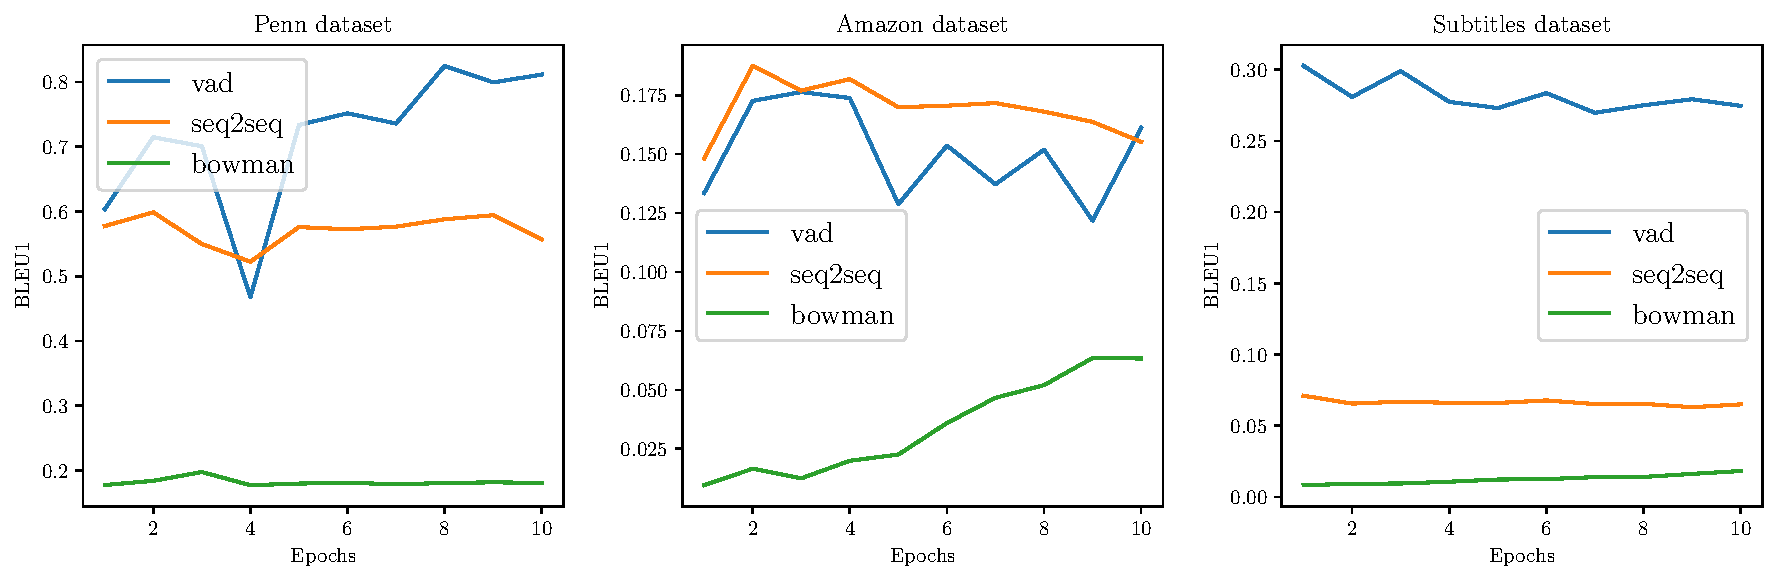
\includegraphics[width=150mm]{results/bleu1.pdf}
	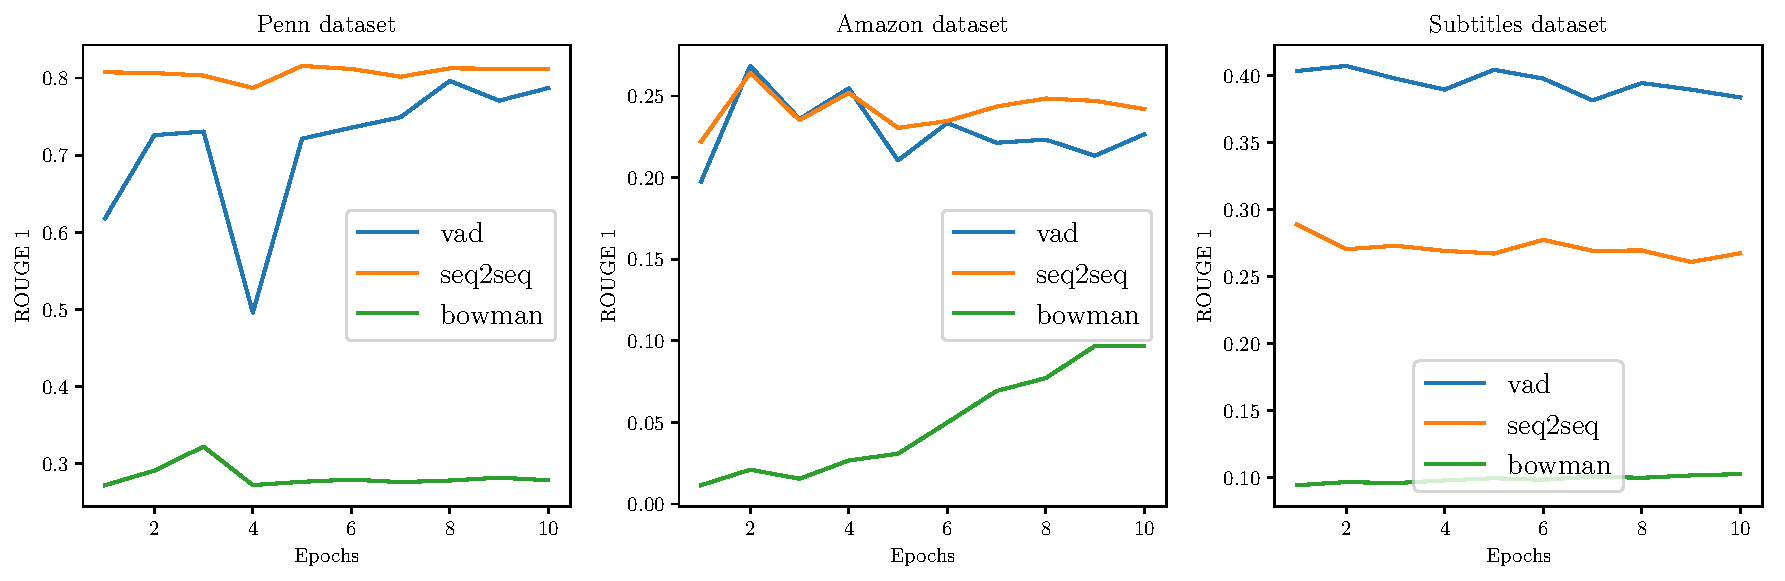
\includegraphics[width=150mm]{results/rouge_1.pdf}
	\caption{BLEU and rouge scores across the three models; higher is better.\label{r:bleu_rouge}}
  \end{figure}

% what is it? how is it measured? what does it say

\section{F1}

\begin{figure}[!ht]
	\centering
	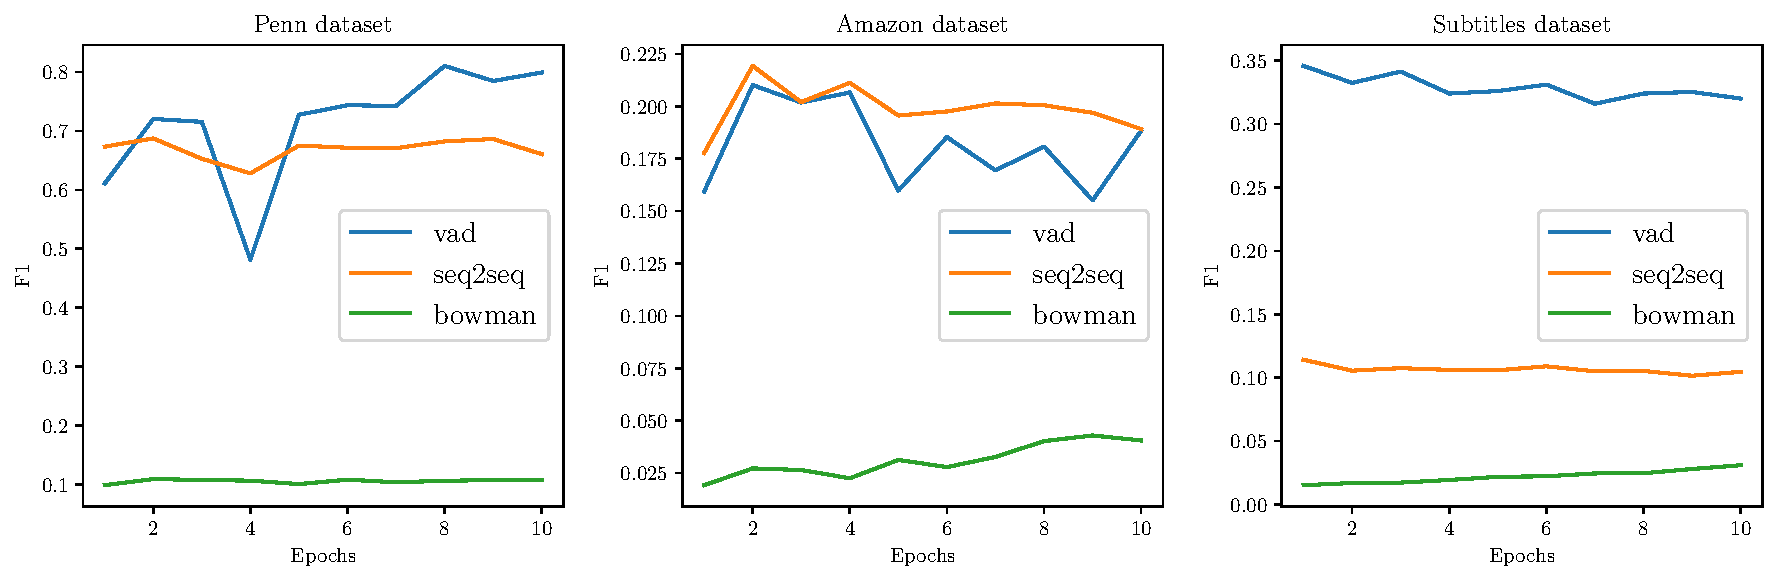
\includegraphics[width=150mm]{results/f1.pdf}
	\caption{F1 scores across the three models; higher is better.\label{r:f1}}
  \end{figure}

% what is it? how is it measured? what does it say

\section{Output Variance}

The motive of the responses is to 
The responses produced here should com

\section{Sampling Examples}

In additional to quantitiative measurements, we also generate example resonses 
As some of our models are based on bayesian inference, we sample five outputs and hand pick the most optimal responses out of each of the relevant models. 

\chapter{Future Work}

One of the caveats of a research is typically that research direction is open ended. 
- talk about how you could potentially increase the KL weight by merging the SBOW with the reconstruction loss

- use nn to classify performance of outputs to detect realisticness of data
- apply to gan to improve model performance
- more measurements
- BLEU/ROUGE against the most optimal solution but requires extensive memory usage and would take a considerably longer running time due to technical implementation.
- longer Hyperparameter optimisation
- augment amazon reviews s.t. the item ID is the mean of the item weights.
- explore completely generative sequences end to end.

% %%%%%%%%%%%%%%%%%%%%%%%%%%%%%%%%%%%%
\chapter{Conclusion}

% In conclusion, we identified the one-to-many nature of open-domain conversation and proposed two novel models that show superior performance in generating diverse and appropriate responses at the discourse level. While the current paper addresses diversifying responses in respect to dialogue acts, this work is part of a larger research direction that targets leveraging both past linguistic findings and the learning power of deep neural networks to learn better representation of the latent factors in dialog. In turn, the output of this novel neural dialog model will be easier to explain and control by humans. In addition to dialog acts, we plan to apply our kgCVAE model to capture other different linguistic phenomena including sentiment, named entities,etc. Last but not least, the recognition network in our model will serve as the foundation for designing a data driven dialog manager, which automatically discovers useful high-level intents. All of the above suggest a promising research direction.

In this paper, 
%In this paper, a novel variational autoregressive decoder is proposed to improve the performance of VAE-based models for open-domain response generation. By injecting the variational inference into the RNN-based decoder and applying carefully designed conditional variables and auxiliary objective for latent variables, the proposed model is expected to better modeling semantic informa- tion of text in conversations. Quantitative and qualitative experimental results show clear perfor- mance improvement of the proposed model over competitive baselines. In future works, we will explore the use of other attributes of responses such as Part-of-Speech (POS) tags and chunking sequences as additional conditions for better re- sponse generation.

- generated responses may not necessarily be indicative of the data is is modelled against.
- kl loss is difficult to develop (although there are many attempts at this)
- vad has more kl weight (which is natural)
- outputs are more varied with vad (again based on the kl weight)
- regular vaes on seq2seq networks are great but requires lots of hyperparameter tuning

In no necessary surpise

When VAEs are trained with powerful decoders, the model can learn to ‘ignore the latent variable’. This isn’t something an autoencoder should do. 

However, with the advent of Transformer models (\cite{chromiak_transformer_2017}), and most notably the introduction of 


%% bibliography
\bibliographystyle{apa}
\bibliography{ref} 

\chapter*{Appendix}

\section{KL Divergence Derivation}
\label{kl_derivation}
Let $\mu_1, \sigma_1 \rightarrow \mathcal{N}(\mu_1,\sigma_1)$ be our first distribution, and $\mu_2, \sigma_2 \rightarrow \mathcal{N}(\mu_2,\sigma_2)$ be our second distribution. By deriving this, we would be able to calculate a derivative friendly loss function for our models.

\begin{equation}
	\label{eq:t}
	\begin{aligned}
	KL &= \int \left[\log( p(x)) - \log( q(x)) \right]\ p(x)\ dx \\
	% &= \frac{1}{2}\left[\log\frac{|\Sigma_2|}{|\Sigma_1|} - d + tr(\Sigma_2^{-1}\Sigma_1) + (\mu_2 - \mu_1)^T \Sigma_2^{-1}(\mu_2 - \mu_1)\right] \\
	&= \int \left[ \frac{1}{2} \log\frac{|\Sigma_2|}{|\Sigma_1|} - \frac{1}{2} (x-\mu_1)^T\Sigma_1^{-1}(x-\mu_1) + \frac{1}{2} (x-\mu_2)^T\Sigma_2^{-1}(x-\mu_2) \right] \times p(x) dx \\
	&= \frac{1}{2} \log\frac{|\Sigma_2|}{|\Sigma_1|} - \frac{1}{2} \text{tr}\ \left\{E[(x - \mu_1)(x - \mu_1)^T] \ \Sigma_1^{-1} \right\} + \frac{1}{2} E[(x - \mu_2)^T \Sigma_2^{-1} (x - \mu_2)] \\
	&= \frac{1}{2} \log\frac{|\Sigma_2|}{|\Sigma_1|} - \frac{1}{2} \text{tr}\ \{I_d \} + \frac{1}{2} (\mu_1 - \mu_2)^T \Sigma_2^{-1} (\mu_1 - \mu_2) + \frac{1}{2} \text{tr} \{ \Sigma_2^{-1} \Sigma_1 \} \\
	&= \frac{1}{2}\left[\log\frac{|\Sigma_2|}{|\Sigma_1|} - d + \text{tr} \{ \Sigma_2^{-1}\Sigma_1 \} + (\mu_2 - \mu_1)^T \Sigma_2^{-1}(\mu_2 - \mu_1)\right].
\end{aligned}
\end{equation}

\end{document}
